\documentclass{report}
\usepackage[utf8]{inputenc}
\usepackage{graphicx}
\graphicspath{ {images/} }

\title{First Document}
\author{Jiayi Hu}

\begin{document}

\maketitle

\tableofcontents

\begin{abstract}
	This is a simple paragraph at the beginning of the document. A brief introduction about the main subject.
\end{abstract}

\begin{figure}[h]
	\centering
	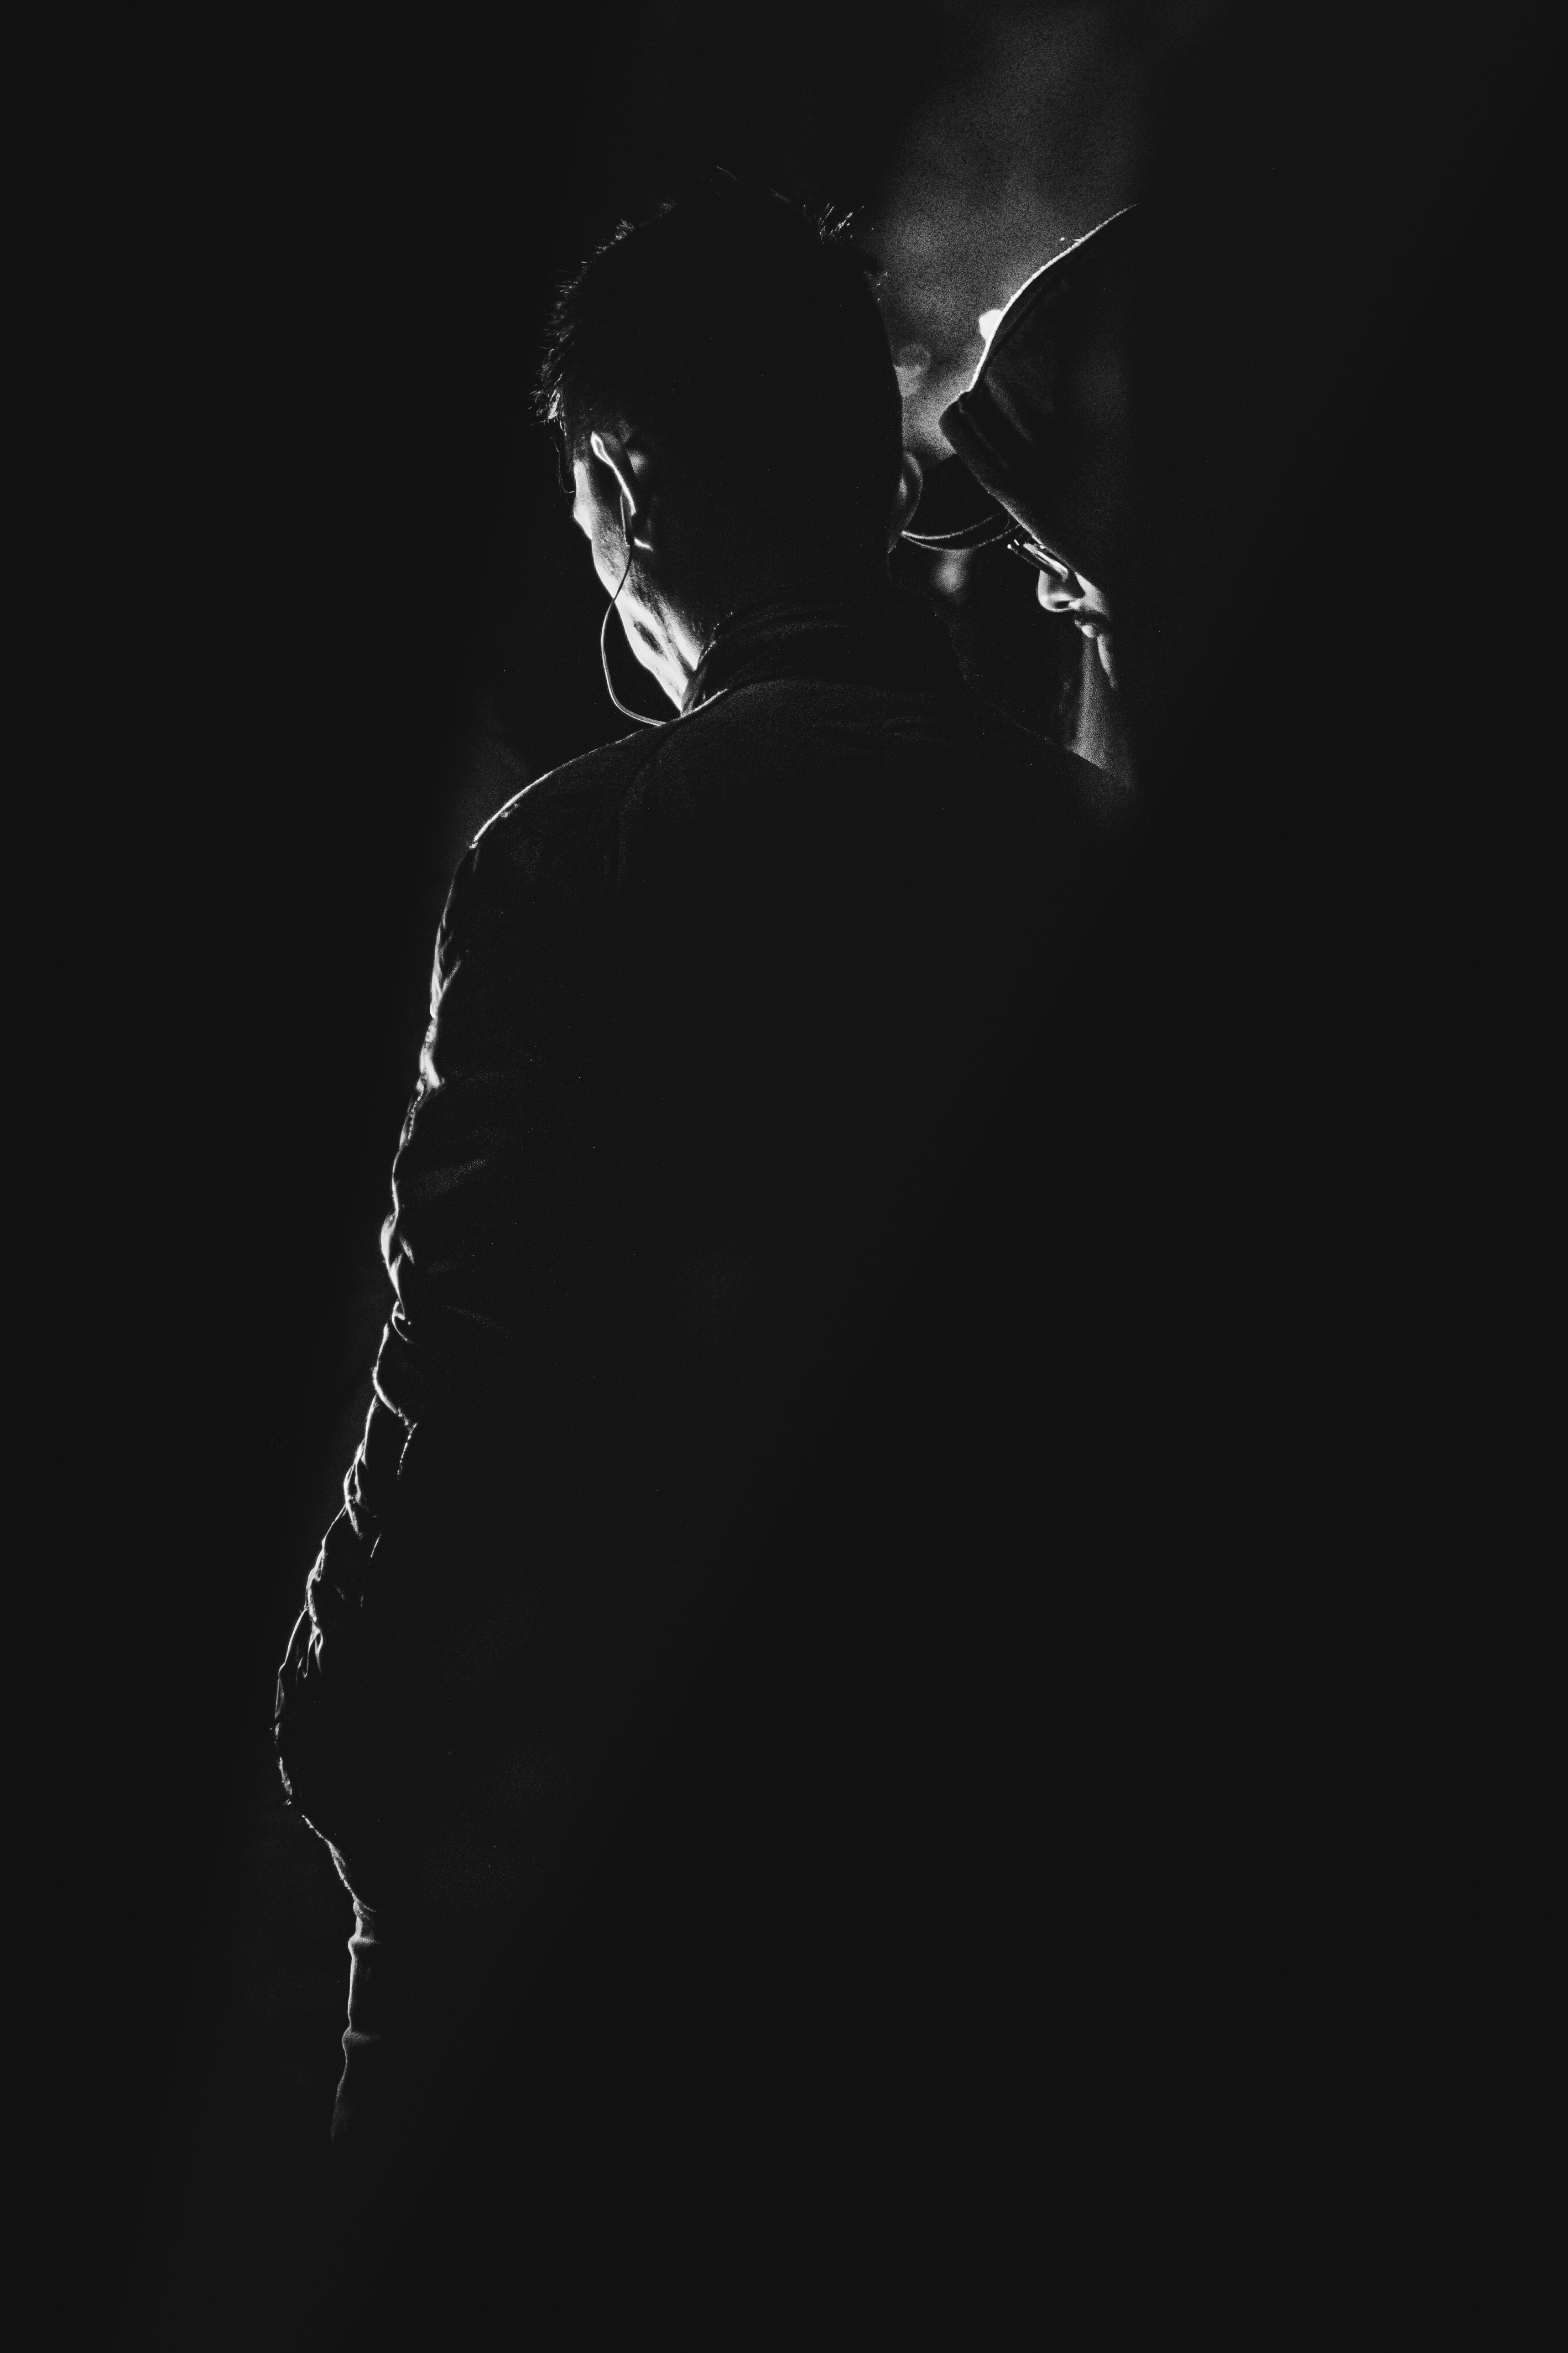
\includegraphics[width=0.25\textwidth]{private}
	\caption{a nice private investigator}
	\label{fig:mesh1}
\end{figure}

As you can see in the figure \ref{fig:mesh1}, the function grows near 0. Also, in the page \pageref{fig:mesh1} is the same example.

% Comment
First document. This is a simple example, with no 
extra parameters or packages included. \\

Some of the \textbf{greatest} discoveries in \underline{science} were made by \textbf{\textit{accident}}

\begin{itemize}
	\item The individual entries are indicated with a black dot, a so-called bullet.
	\item The text in the entries may be of any length.
\end{itemize}

\begin{enumerate}
	\item This is the first entry in our list
	\item The list numbers increase with each entry we add
\end{enumerate}

\chapter{First Chapter}

\section{Introduction}

This is the first section.

Lorem  ipsum  dolor  sit  amet,  consectetuer  adipiscing  
elit.   Etiam  lobortisfacilisis sem.  Nullam nec mi et 
neque pharetra sollicitudin.  Praesent imperdietmi nec ante. 
Donec ullamcorper, felis non sodales...


\section{Second Section}

Lorem  ipsum  dolor  sit  amet,  consectetuer  adipiscing  
elit.   Etiam  lobortisfacilisis sem.  Nullam nec mi et 
neque pharetra sollicitudin.  Praesent imperdietmi nec ante. 
Donec ullamcorper, felis non sodales...

\subsection{First Subsection}
Praesent imperdietmi nec ante. Donec ullamcorper, felis non sodales..

\addcontentsline{toc}{section}{Unnumbered Section}
\section*{Unnumbered Section}
Lorem  ipsum  dolor  sit  amet,  consectetuer  adipiscing  
elit



\end{document}